\documentclass[Thesis.tex]{subfiles}
\begin{document}

\chapter{{\sc ConformalLab} - Conformal maps and uniformization}
\label{chp:conformallab}

\section{Data format}
To store and process data {\sc ConformalLab} uses an {\sc XML} data format.
All examples presented in Chapter~\ref{chp:conformal_examples} are stored
in this format. 


\subsection{Schottky data} 


A Riemann surface can be given by Schottky data, see Section~\ref{sec:schottky_examples}. An example is shown in Listing~\ref{lst:schottky_xml}. {\tt SchottkyData} can include one ro more {\tt SchottkyGenerator}s. A {\tt SchottkyGenerator} defines the fix points $A$ and $B$, the complex number $\mu$, and a {\tt Circle}. This circle is required to contain $A$ and must not contain $B$.

\begin{lstlisting}[label=lst:schottky_xml, caption={Schotty data}, numbers=none, language=XML, captionpos=b]
<SchottkyData xmlns="http://www.varylab.com/conformallab/types" name="Schottky">
    <SchottkyGenerator>
        <A re="-1.0" im="0.0"/>
        <B re="1.0" im="0.0"/>
        <Mu re="0.25" im="0.0"/>
        <Circle radius="1.33333333333333">
            <Center re="-1.66666666666666" im="0.0"/>
        </Circle>
    </SchottkyGenerator>
</SchottkyData>
\end{lstlisting}


\section{User interface}
\begin{figure}
\centering
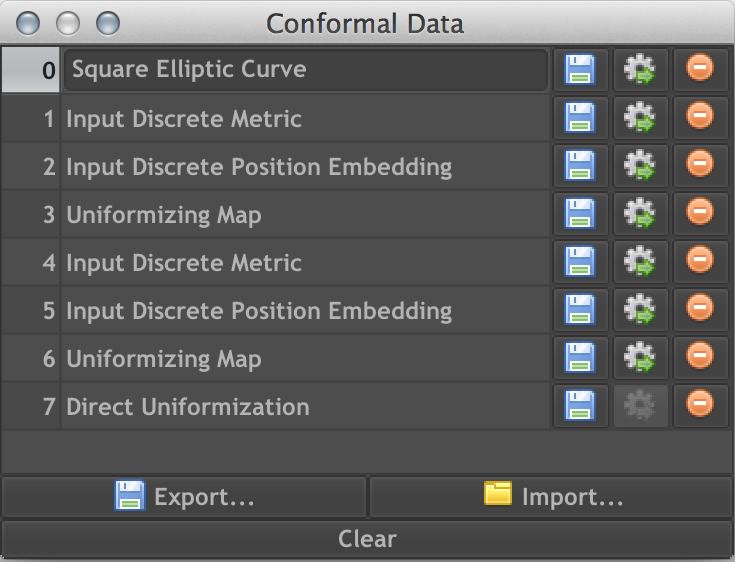
\includegraphics[width=0.4\linewidth]{conformllab/conformal_data.png}
\caption{XML data import and export interface of {\sc ConformalLab}.}
\label{fig:conformal_data}
\end{figure}

\begin{figure}
\centering
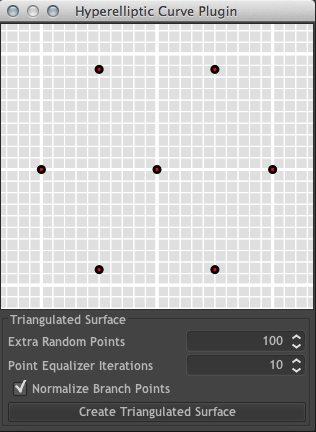
\includegraphics[width=0.25\linewidth]{conformllab/hyperelliptic_curve.png}
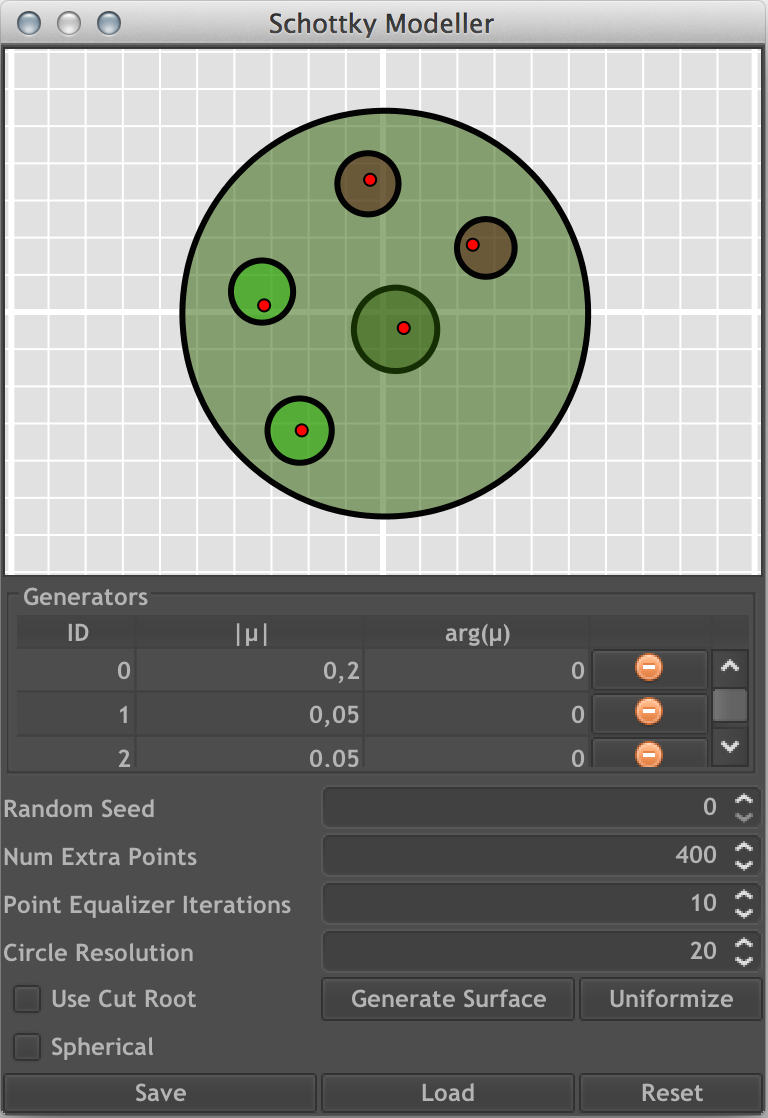
\includegraphics[width=0.3\linewidth]{conformllab/schottky_modeller.png}
\caption{Hyperelliptic curve interface and the Schottky modeller user interface
of {\sc ConformalLab}.}
\label{fig:conformal_data}
\end{figure}

\begin{figure}
\centering
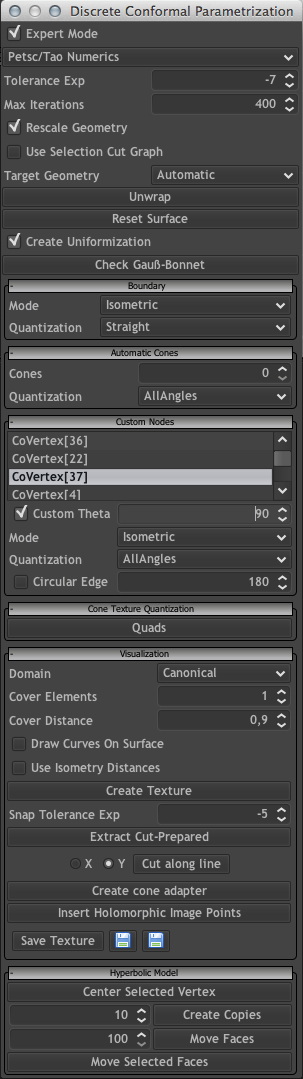
\includegraphics[width=0.3\linewidth]{conformllab/main_interface.png}
\caption{Hyperelliptic curve interface and the Schottky modeller user interface
of {\sc ConformalLab}.}
\label{fig:conformal_data}
\end{figure}



\subfilebibliography
\end{document}

%%% Local Variables:
%%% TeX-master: "Thesis.tex"
%%% End: